\documentclass[12pt]{article}

% Packages for formatting
\usepackage[margin=1in]{geometry}
\usepackage{titlesec}
\usepackage{enumitem}
\usepackage{xcolor}
\usepackage{graphicx} % for including images

% Header and footer formatting
\usepackage{fancyhdr}
\pagestyle{fancy}
\fancyhf{}
\rhead{Assignment No 3}
\lhead{Subject: Compiler Construction}
% \chead{Section: BCS-6A, Assignment No. 3}
\rfoot{Page \thepage}

% Section formatting
\titleformat{\section}[block]{\Large\bfseries\filcenter}{}{1em}{}
\titleformat{\subsection}[hang]{\large\bfseries}{}{1em}{}

% List formatting
\setlist[itemize]{leftmargin=*}
\setlist[enumerate]{leftmargin=*}

% Custom colors
\definecolor{myblue}{RGB}{0,95,140}
\definecolor{mygray}{RGB}{175,175,175}

\begin{document}

\begin{center}
{\LARGE\bfseries Compiler Construction Assignment \#3}\\[0.5em]
{\large Name: Jawad Ahmed}\\[0.5em]
{\large Section: BCS-6A}\\[0.5em]
{\large Instructor: Usman Wajid}\\[0.5em]
\end{center}

\section{Instructions}
\begin{itemize}
\item Rewrite the lexical analyzer code (in assignment 02) in Lex tool (Latest version Flex)
\item Submit only the Lex file as your assignment
\item Also submit the screen shot of your output
\item Your assignment  02 and assignment  03 should link with each other
\end{itemize}

\section{Lex Code}
The lex code is shown in fiqure 1.
\begin{figure}[htbp]
  \centering
  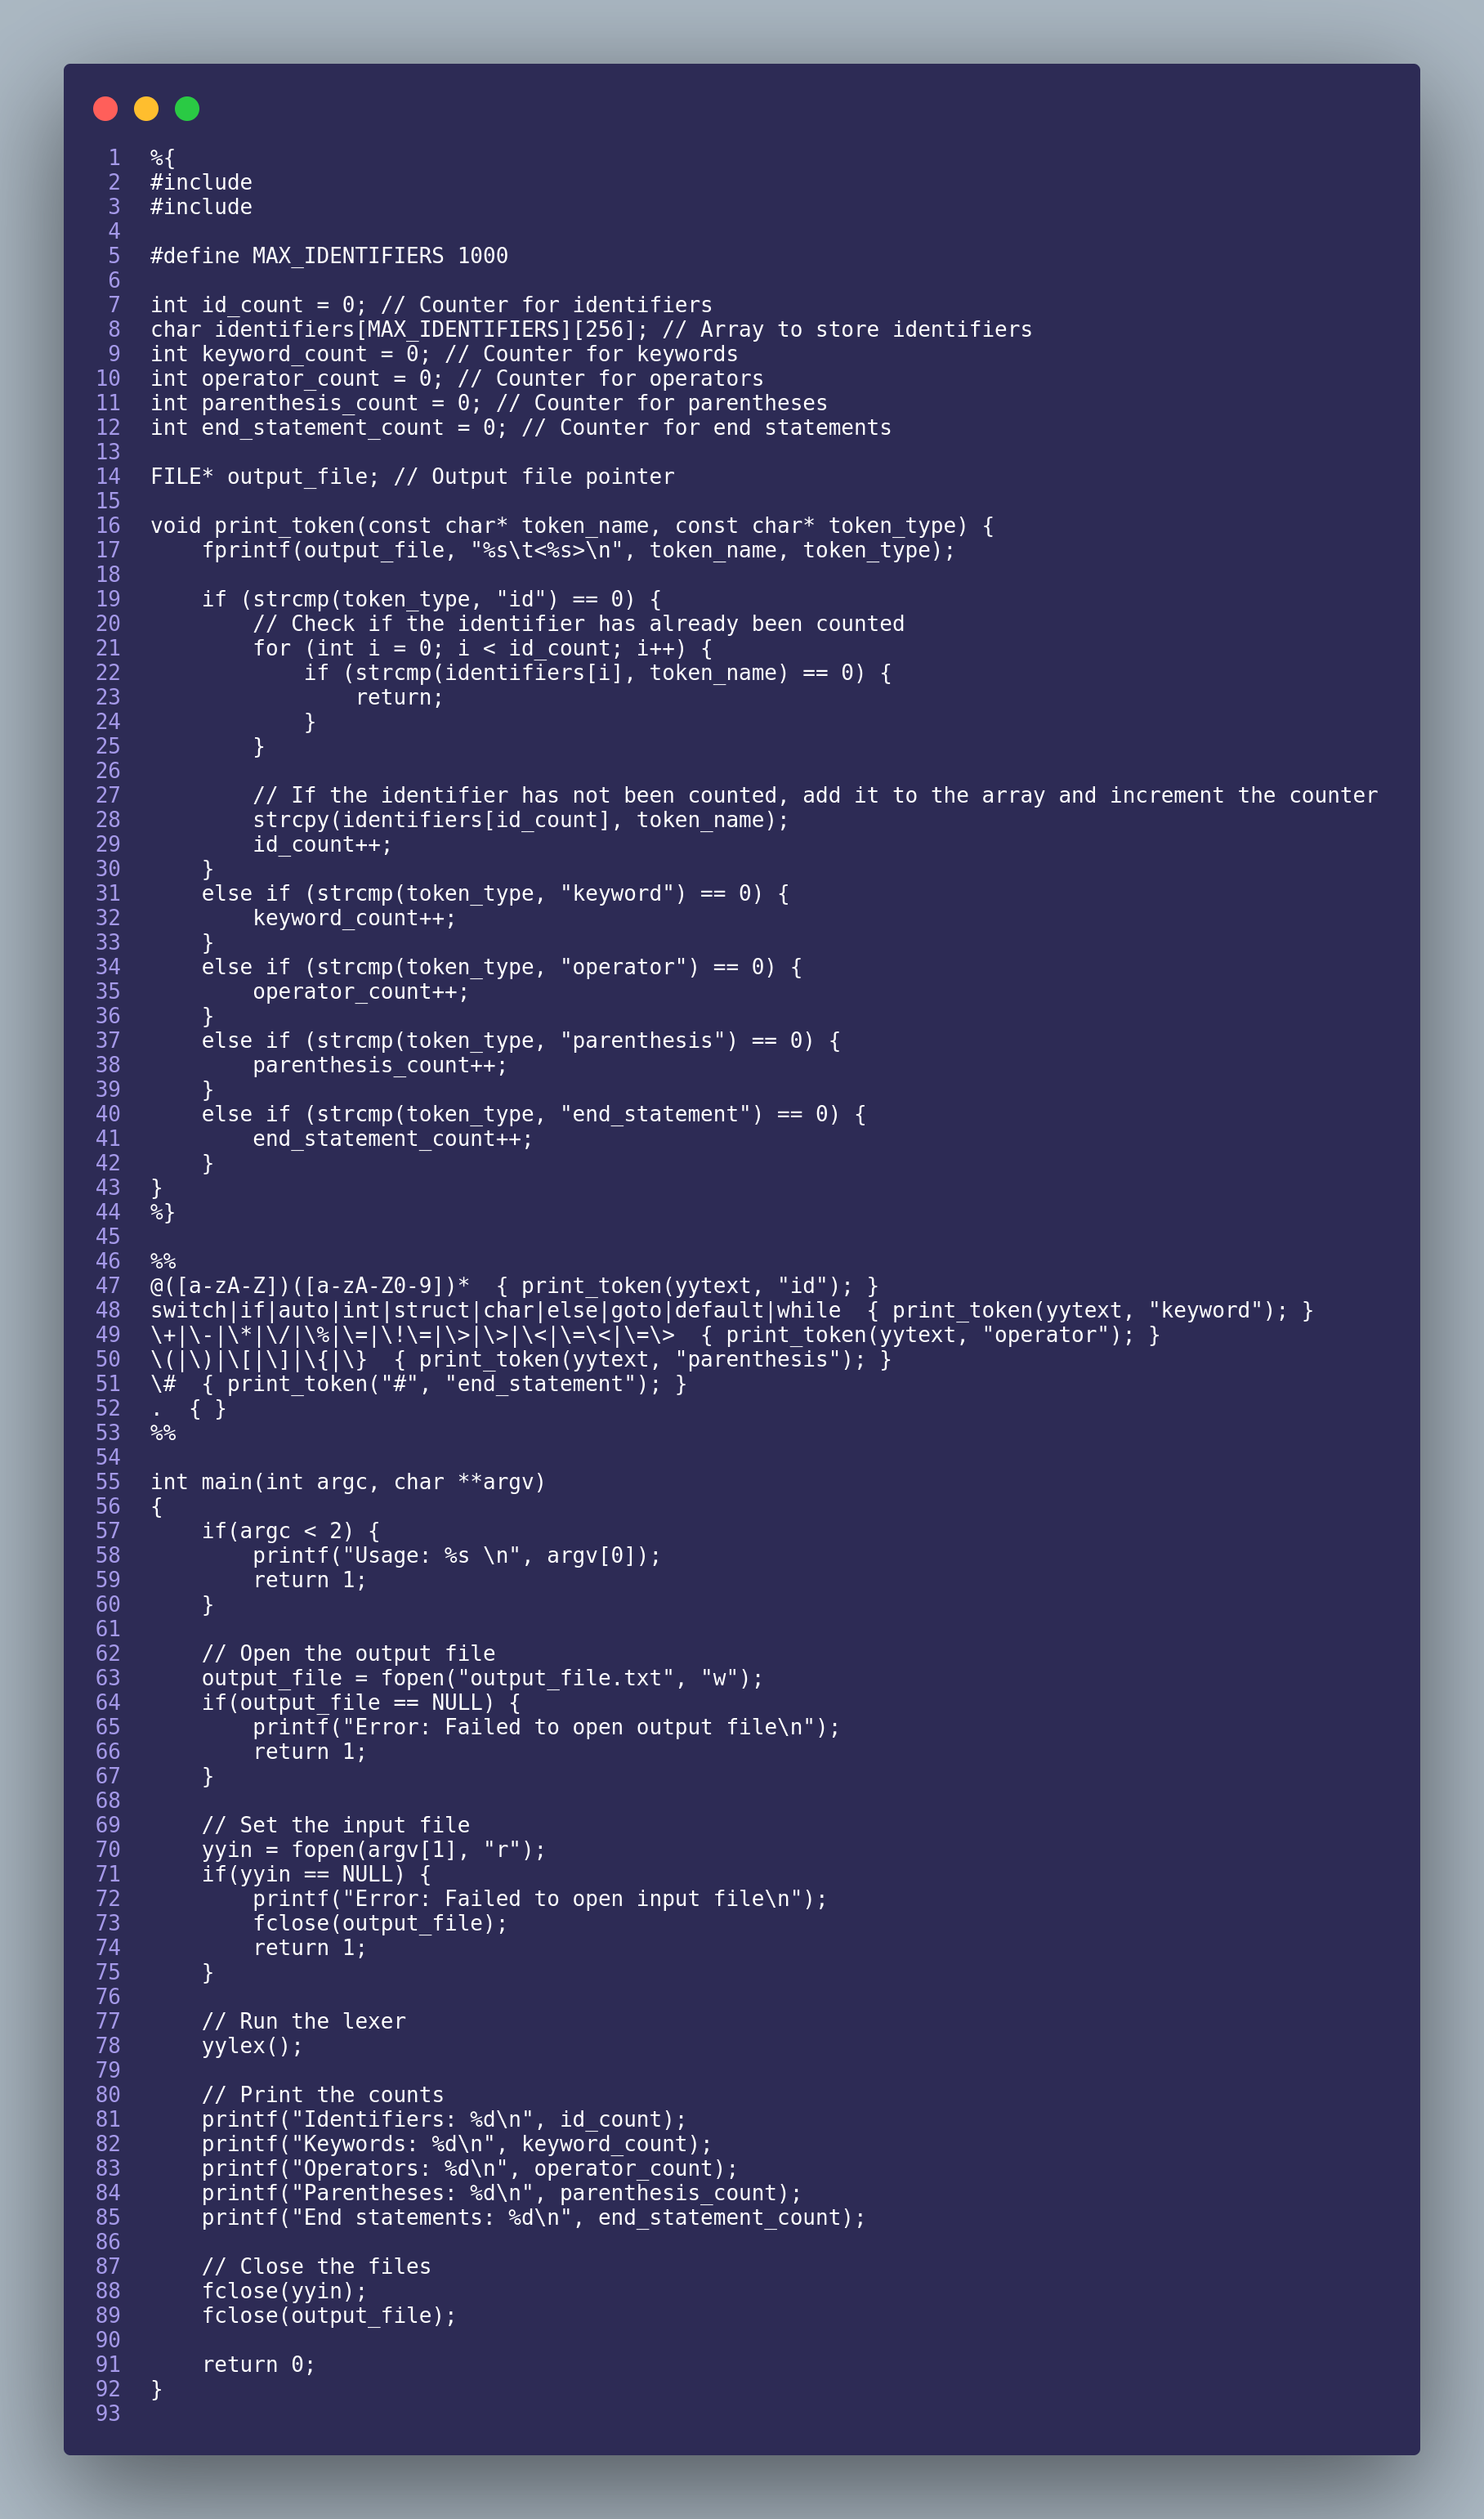
\includegraphics[width=0.8\textwidth]{code.png}
  \caption{Lex Code}
  \label{fig:example}
\end{figure}

\section{Output}
\subsection{Inputfile}
The contents of the input file is shown in figure 2.
\begin{figure}[htbp]
  \centering
  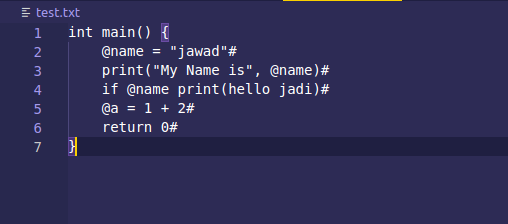
\includegraphics[width=0.8\textwidth]{sample_input.png}
  \caption{Input File}
  \label{fig:example}
\end{figure}
\subsection{Output Of the code}
The output given by the above lex code is given in figure 3.
\begin{figure}[htbp]
  \centering
  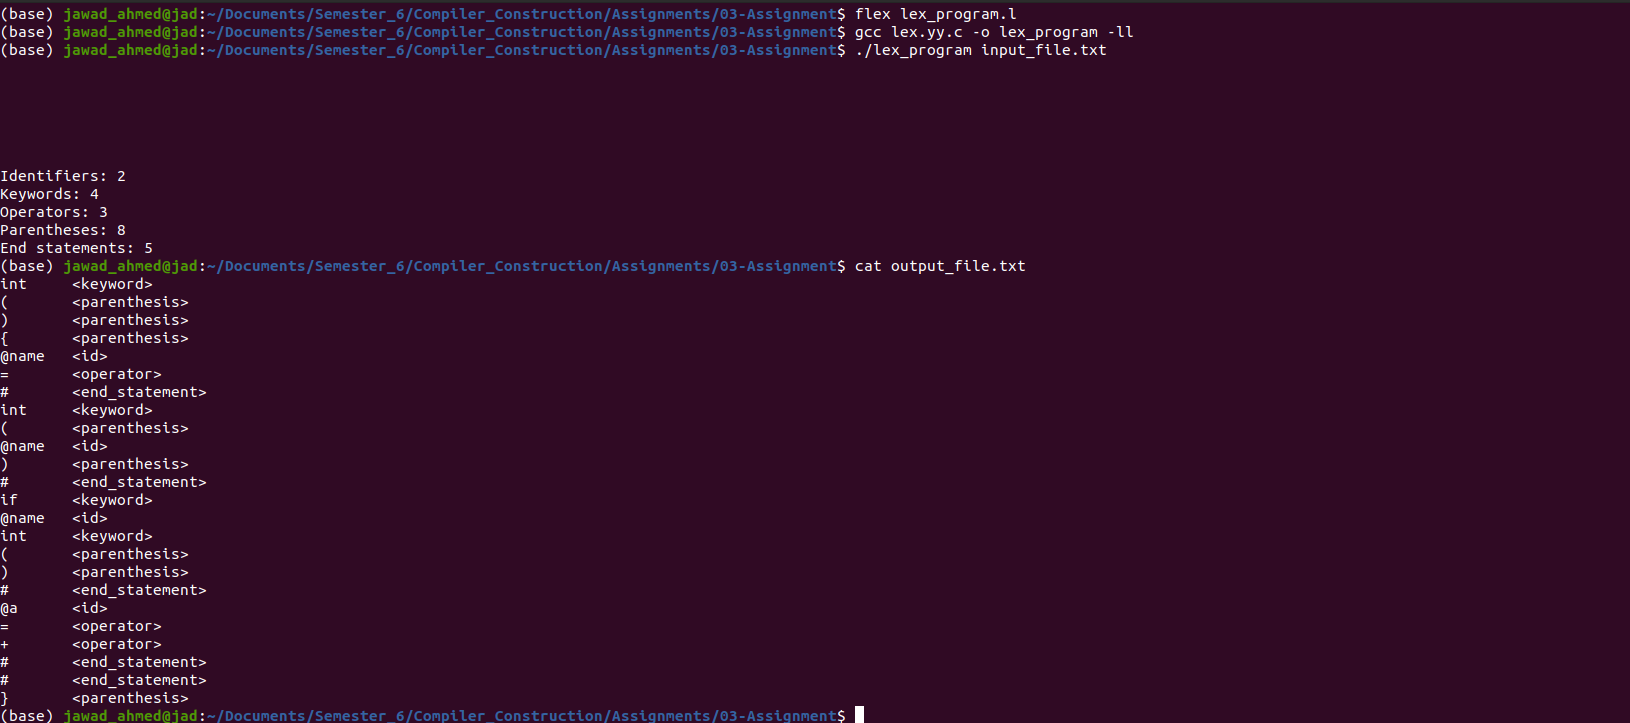
\includegraphics[width=1\textwidth]{code-output.png}
  \caption{Output}
  \label{fig:example}
\end{figure}

\end{document}
